\chapter{统计力学}
\section{玻尔兹曼分布}
先考虑这样一个问题:假设空气的温度是均匀的,那么空气的密度和压强随高度怎么分布呢?

如图\ref{fig-air-block},在高度为$h$处取一小块底面积为$\Delta S$,高度为$\Delta h$的空气作为研究对象,设它的密度为$\rho$,那么它的质量就是$\rho \Delta S \Delta h$,上下受到的压强分别是$p(h+\Delta h)$和$p(h)$。
\begin{figure}[htb]
\centering
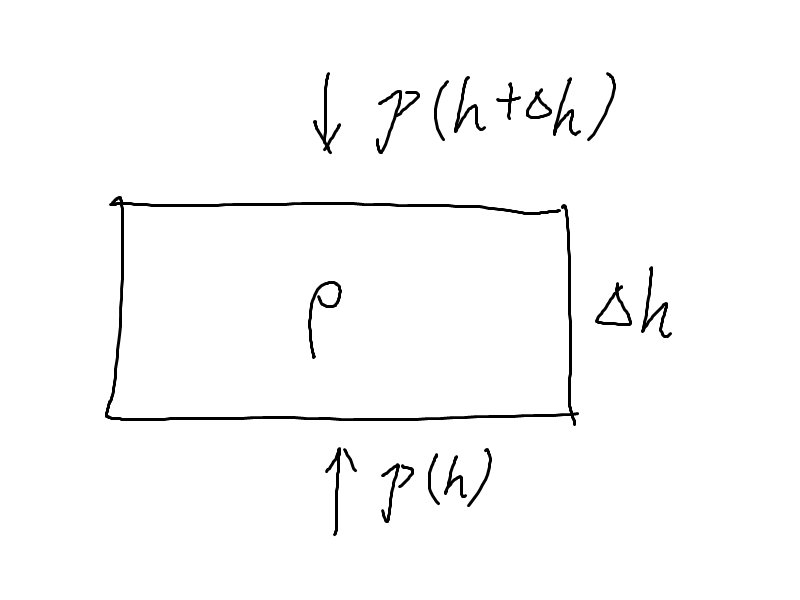
\includegraphics[scale=0.5]{fig/air-block.png}
\caption{一块空气}
\label{fig-air-block}
\end{figure}

这块空气受力平衡,$\rho \Delta S \Delta h g+p(h+\Delta h) \Delta S-p(h) \Delta S=0$,化简得$\rho g \Delta h+\Delta p=0$。

我们知道理想气体状态方程$p V=n R T$,另一种写法是$p \mu=\rho R T$,$\mu$是空气的平均相对分子质量,设它随高度是不变的。$R$叫作普适气体常量, $R \approx 8.31 \unit{J/(mol \cdot K)}$。两边微分得到$\Delta p \mu=\Delta \rho R T$。

(先不管差分算符$\Delta$和微分算符$\opd$的区别。$\rho(h)$和$p(h)$都是$h$的函数,有时候自变量省略不写)

合起来得到$\frac{\Delta \rho}{\rho}=-\frac{\mu g \Delta h}{R T}$,这是一个关于$\rho(h)$的微分方程,解得$\rho=\rho_0 \rme^{-\frac{\mu g h}{R T}}$。如果$h$是从地面开始算的,那么$\rho_0$就是地面处的空气密度。

温度$T$越高,比例系数$\frac{\mu g}{R T}$越小,指数衰减就越慢,也就是说分子(比温度低的时候)更容易出现在高的地方。(方便起见,这里把分子、原子之类的东西都叫作分子)

一个分子的质量$m=\frac{\mu}{N_A}$,玻尔兹曼常量$k=\frac{R}{N_A}$,所以上式也可以写成$\rho=\rho_0 \rme^{-\frac{m g h}{k T}}$。

代入$p$的式子得到$p=p_0 \rme^{-\frac{m g h}{k T}}$。同理可以得到分子数密度$\frac{\Delta N}{\Delta V}$也符合$\rme^{-\frac{m g h}{k T}}$的分布。也就是说,高度为$h$处出现一个分子的概率正比于$\rme^{-\frac{m g h}{k T}}$。设这个概率为$f_h(h)=A \rme^{-\frac{m g h}{k T}}$,$A$是一个比例系数,这就是分子高度的分布函数,叫作玻尔兹曼分布。

既然它是一个概率,那么各个地方出现分子的概率加起来必须等于$1$,也就是$\int_0^\infty f_h(h) \opd h=1$,所以$A=\frac{m g}{k T}$。这种乘上一个常数,让概率加起来等于$1$的方法叫作\emph{归一化}。
\section{麦克斯韦分布}
现在考虑分子速度的分布。速度有$x,y,z$三个分量,先考虑$z$分量。如果高度为$0$的地方有一个分子的$v_z$为$v_{z 0}$,那么它可以跑到高度为$\frac{v_{z 0}^2}{2 g}$的地方,并且$v_z$变为$0$。(只考虑重力作用,忽略分子之间的作用)

也就是说,$v_z$为$v_{z 0}$,高度为$0$的分子数等于$v_z$为$0$,高度为$\frac{v_{z 0}^2}{2 g}$的分子数。设分子的$v_z$和高度的分布函数为$f_{v_z,h}(v_z,h)$,那么$f_{v_z,h}(v_{z 0},0)=f_{v_z,h}(0,\frac{v_{z 0}^2}{2 g})$。

然后麦克斯韦做了一个假设:在不同的高度,分子的速率分布是相同的。如果高度为$1 \unit{m}$的分子中速度为$2 \unit{m/s}$的分子占了$10\%$,那么高度为$10 \unit{m}$的分子中速度为$2 \unit{m/s}$的分子也占$10\%$。因此分布函数可以表示为$f_{v_z,h}(v_z,h)=f_{v_z}(v_z) f_h(h)$,$f_{v_z}$和$f_h$是两个独立的分布函数,现在需要求出$f_{v_z}$。

$f_{v_z}(v_{z 0}) f_h(0)=f_{v_z}(0) f_h(\frac{v_{z 0}^2}{2 g})$,代入已知的$f_h$得到$f_{v_z}(v_{z 0})=f_{v_z}(0) \rme^{-\frac{m g}{k T} \frac{v_{z 0}^2}{2 g}}$,也就是说$f_{v_z}(v_z)=f_{v_z}(0) \rme^{-\frac{m v_z^2}{2 k T}}$。

现在$f_{v_z}(0)$相当于一个待定的比例系数,要让$\int_{-\infty}^\infty f_{v_z}(v_z) \opd v_z=1$。(刚才是从$0$积到$\infty$,因为分子的高度是从$0$开始算的;现在是从$-\infty$积到$\infty$,因为分子的$v_z$可正可负)

计算这个积分比较困难,这里直接给出结论:$\int_{-\infty}^\infty \rme^{-x^2} \opd x=\sqrt{\pi}$,所以$\int_{-\infty}^\infty f_{v_z}(0) \rme^{-\frac{m v_z^2}{2 k T}} \opd v_z=\sqrt{\pi} \sqrt{\frac{2 k T}{m}} f_{v_z}(0)$,$f_{v_z}(0)=\sqrt{\frac{m}{2 \pi k T}}$。

(现在这些奇怪的积分如果不会算没关系,也用不着背下来,会算一些最简单的积分就行了)

$f_{v_z}$只包含$v_z$的二次项,所以$+v_z$和$-v_z$对应的$f_{v_z}$是一样的。许多只与速度的大小有关,而与方向无关的东西可以用这一点来检查。

向各个方向运动的分子数是均匀的,所以$f_{v_x}$和$f_{v_y}$应该与$f_{v_z}$一样:$f_{v_x}(v_x)=\sqrt{\frac{m}{2 \pi k T}} \rme^{-\frac{m v_x^2}{2 k T}}$,$f_{v_y}(v_y)=\sqrt{\frac{m}{2 \pi k T}} \rme^{-\frac{m v_y^2}{2 k T}}$。

把它们乘起来得到$f_{v_x,v_y,v_z}(v_x,v_y,v_z)=(\frac{m}{2 \pi k T})^\frac{3}{2} \rme^{-\frac{1}{k T} \frac{1}{2} m (v_x^2+v_y^2+v_z^2)}$$=(\frac{m}{2 \pi k T})^\frac{3}{2} \rme^{-\frac{m v^2}{2 k T}}$,这就是分子速度(包括三个分量,或者说大小和方向)的分布函数。

前面的系数目前不是很重要,重要的是后面是一个指数衰减$\rme^{-\frac{m v^2}{2 k T}}$。

如果只考虑速度的大小(速率),可以取一个坐标轴为$v_x,v_y,v_z$的三维坐标系,把分子按照速度放在坐标系里。然后画一个以原点为中心,$v$为半径的球面,面积为$4 \pi v^2$。这个球面上的分子都满足速率为$v$,而球面上的每一点的分子数密度为$(\frac{m}{2 \pi k T})^\frac{3}{2} \rme^{-\frac{m v^2}{2 k T}}$,所以分子速率的分布函数$f_v(v)=4 \pi v^2 (\frac{m}{2 \pi k T})^\frac{3}{2} \rme^{-\frac{m v^2}{2 k T}}$。这就是麦克斯韦速率分布。

如果分子的坐标是$x,y,z$,对应的速度是$\dot x,\dot y,\dot z$,那么把坐标的分布函数和速度的分布函数乘起来就能得到“坐标和速度”的分布函数$f(x,y,z,\dot x,\dot y,\dot z)=\frac{m g}{k T} (\frac{m}{2 \pi k T})^\frac{3}{2} \rme^{-\frac{1}{k T} (\frac{1}{2} m (\dot x^2+\dot y^2+\dot z^2)+m g z)}$。
\section{分布函数}
可以发现,分子高度的分布函数有一项$\rme^{-\frac{m g h}{k T}}$,速度的分布函数有一项$\rme^{-\frac{m v^2}{2 k T}}$。现在可以猜:如果一个分子的坐标是$q$(多个坐标的情况类似),速度是$\dot q$,能量是$E(q,\dot q)$,那么分布函数就是$f(q,\dot q)=A \rme^{-\frac{E}{k T}}$,$A$是归一化系数。

如果一个系统(专业一点叫\emph{系综})里有很多一样的分子,忽略这些分子之间的相互作用,并且系统达到热平衡,那么从里面随便取一个分子,它的坐标为$q_0$,速度为$\dot q_0$的概率就是$f(q_0,\dot q_0)$。可以看出,温度越高,指数衰减越慢,分子越容易具有较高的能量。

(现在把这一点当作基本假设,但是严格的统计力学是用别的基本假设推出它的。而且它只对温度和分子数恒定的系统成立)

什么叫热平衡?这个问题现在先不仔细讲。在空气的例子中,热平衡就是各处的温度相同,而且随便取一小块空气都受力平衡。系统要达到热平衡,那么分子之间的相互作用不可能完全为零,否则热量就不能从一部分传到另一部分。分子之间的相互作用不可忽略,或者系统没有达到热平衡的情况比较复杂,我们也不仔细讲。
\section{统计平均值}
知道分布函数之后,可以算出分子微观性质的统计平均值,它就是物质的宏观性质。

比如空气的例子中,我们来计算分子的平均高度:$\overline{h}=\int_0^\infty h f_h(h) \opd h=\int_0^\infty h \frac{m g}{k T} \rme^{-\frac{m g h}{k T}} \opd h$。这个积分我们可以学一下:
\begin{align*}
\int_0^\infty x \rme^{-x} \opd x&=\int_0^\infty x \cdot (-\opd \rme^{-x}) \\
&=\left. -x \rme^{-x} \right|_0^\infty-\int_0^\infty (-\rme^{-x}) \opd x \\
&=\left. -x \rme^{-x} \right|_0^\infty-\left. \rme^{-x} \right|_0^\infty \\
&=1
\end{align*}

令$x=\frac{m g h}{k T}$,得到$\overline{h}=\frac{k T}{m g}$。还可以算出平均重力势能$\overline{E}=\int_0^\infty m g h f_h(h) \opd h=k T$。这是从地面到无穷高处的空气的平均重力势能,而且作了很多并不实际的简化。一般我们考虑一个小容器里的气体时,重力势能是忽略的。

只考虑分子在$x$方向上的运动,可以计算平均动能:$\overline{E_{k x}}=\int_{-\infty}^\infty \frac{1}{2} m v_x^2 f_{v_x}(v_x) \opd v_x$。计算这个积分也比较困难,这里直接给出结论:$\overline{E_{k x}}=\frac{1}{2} k T$。

类似地有$\overline{E_{k x}}=\overline{E_{k y}}=\frac{1}{2} k T$,三维空间中的平均动能$\overline{E_k}=\frac{3}{2} k T$。也就是说,每个平动自由度对应着$\frac{1}{2} k T$的平均动能。

一摩尔气体的能量$E_\text{mol}=N_A \overline{E_k}=\frac{3}{2} R T$。它的比热是升高单位温度需要的能量,所以比热$C_\text{mol}=\frac{\opd E_\text{mol}}{\opd T}=\frac{3}{2} R$。对于只能平动,不能转动的单原子分子,这个结果与实验基本符合,更精确的结果需要考虑量子效应。
\section{量子谐振子}
上面考虑的都是坐标和能量可以连续分布的情况,但是在量子力学中,能量是离散(不连续)分布的,这时把上面的积分改成求和就行了。

固体里的分子在平衡位置附近振动,它们的能量可以取$\hbar \omega,2 \hbar \omega,3 \hbar \omega,\dots$,$\hbar \omega$是一个单位的能量。分子的能量为$n \hbar \omega$的概率$f(n)=A \rme^{-\frac{n \hbar \omega}{k T}}$。

然后确定$A$:$\sum_{n=1}^\infty f(n)=A \frac{\rme^{-\frac{\hbar \omega}{k T}}}{1-\rme^{-\frac{\hbar \omega}{k T}}}$(高考范围内的等比数列求和),而$\sum_{n=1}^\infty f(n)=1$,所以$A=\rme^{\frac{\hbar \omega}{k T}}-1$。

计算一个振子的平均能量:
\begin{align*}
\overline{E}&=\sum_{n=1}^\infty n \hbar \omega f(n) \\
&=A k T \sum_{n=1}^\infty \frac{n \hbar \omega}{k T} \rme^{-\frac{n \hbar \omega}{k T}} \\
&=A k T \frac{\hbar \omega}{k T} \frac{\rme^{-\frac{\hbar \omega}{k T}}}{(1-\rme^{-\frac{\hbar \omega}{k T}})^2} \\
&=\frac{\hbar \omega}{1-\rme^{-\frac{\hbar \omega}{k T}}}
\end{align*}

($\sum n \rme^{-n}$这样的求和应该也是高考范围内的,但是它有一种黑科技的计算方法:先算出$\sum \rme^{-n x}$,然后发现$\sum n \rme^{-n}=-\left. \ddx \sum \rme^{-n x} \right|_{x=1}$。类似的黑科技在后面数列那一章会讲)

一个振子的比热
\begin{equation*}
C=\frac{\opd \overline{E}}{\opd T}=k (\frac{\hbar \omega}{k T})^2 \frac{\rme^{-\frac{\hbar \omega}{k T}}}{(1-e^{-\frac{\hbar \omega}{k T}})^2}
\end{equation*}

比热随温度的变化如图\ref{fig-quant-osc-c}:
\begin{figure}[htb]
\centering
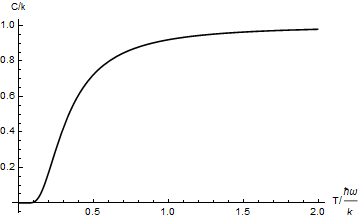
\includegraphics[scale=0.5]{fig/quant-osc-c.png}
\caption{越来越热的时候}
\label{fig-quant-osc-c}
\end{figure}

我们知道$\hbar$很小,而一般情况下$T$很大(物理学中的温度一般是开尔文而不是摄氏度),也就是说$\frac{\hbar \omega}{k T} \ll 1$,$\rme^{-\frac{\hbar \omega}{k T}}=1-\frac{\hbar \omega}{k T}$,做一些小量运算可以得到$\overline{E}=k T$,$C=k$,这与经典理论(比如刚才空气按高度分布)是一致的。如果温度很低,就要考虑量子效应。

总而言之,统计力学就是先想办法确定系统的分布函数,然后计算分子微观性质的统计平均值,得到物质的宏观性质。比如很多电荷定向移动形成电流,很多有磁性的分子有序排列形成磁铁。从力学观点来看,每个分子的运动决定了物质宏观的运动,但是分子太多了,不可能一个个去解它们的运动方程。然而正是因为分子数很多,可以用统计规律来处理它们。
